\documentclass[11pt]{article}
\usepackage[a4paper,margin=2.4cm]{geometry}
\usepackage{amsmath,amssymb}
\usepackage{graphicx}
\usepackage{booktabs}
\usepackage{caption}
\usepackage{subcaption}
\usepackage[hidelinks]{hyperref}
\usepackage{microtype}
\usepackage{placeins}
\setlength{\parindent}{0pt}
\setlength{\parskip}{5pt}
\captionsetup{font=small,labelfont=bf}
\renewcommand{\arraystretch}{1.12}
\setcounter{topnumber}{3}
\setcounter{bottomnumber}{2}
\setcounter{totalnumber}{4}
\renewcommand{\topfraction}{0.92}
\renewcommand{\bottomfraction}{0.6}
\renewcommand{\textfraction}{0.08}
\renewcommand{\floatpagefraction}{0.75}

\title{\bfseries Xenon recoils, thermal abundance and top-associated\\ missing-momentum constraints on exothermic pseudo-Dirac dark matter}
\author{Author list and affiliations to be confirmed}
\date{\today}

\begin{document}
\maketitle

\begin{abstract}
We study an exothermic pseudo-Dirac dark sector in which a vector mediator couples to quarks with strengths proportional to their masses. A reference xenon recoil yield and the Planck relic abundance determine the dark mass and coupling once the mediator mass and the top coupling are chosen. Scanning fourteen mediator masses between 20 and 200~GeV gives 470 admissible points, each generated separately and passed through the CMS all-hadronic $t\bar t$+MET selection. A 15-bin CLs test at $138\ \mathrm{fb}^{-1}$ nominally excludes 381 of them at 95\% CL and leaves 89; every point at or above 100~GeV is excluded. Between 50 and 90~GeV the excluded region runs from a lower boundary at $g_t\approx0.17$ to the top of the scanned range, at 30 and 40~GeV a second boundary closes it at $g_t\approx2.7$ and $3.0$, and at 20~GeV a single point is nominally excluded within the Monte Carlo uncertainty. Three levels of test support the map: the relic equation solved at both Planck-window edges for all 470 nodes, an approximate rescaling of the signal for the same nodes, and dedicated endpoint samples at four nodes, which show that the efficiency carries no systematic shift beyond its statistical scatter. One node crosses $\mu_{95}=1$ at the window edges, by $0.05\%$. The analysis is an expected-only recast, and its limitations are stated explicitly.

\end{abstract}

\section{Introduction}

In an extended nuclear-recoil window with an exposure of $2.84$ tonne\,yr, the LUX-ZEPLIN (LZ) Collaboration reported a candidate event consistent with a recoil energy of $E_R=248\pm23_{\rm stat}\pm23_{\rm syst}$~keV. Across the models considered by LZ, the excess over the background-only hypothesis reached a local significance of $3.4\sigma$ and a global significance of $2.6\sigma$~\cite{LZ}. A dark sector that releases energy in the scattering, rather than absorbing it, can convert a moderately heavy dark state into an energetic xenon recoil; this exothermic mechanism has been studied as an explanation of both the xenon excess and the Galactic Centre gamma-ray excess~\cite{GHK}, and the specific case of a pseudo-Dirac pair coupled through a leptophobic vector mediator has been confronted with the LZ event and with collider data~\cite{DHX}.

The same interactions that produce the recoil also govern the annihilation rate in the early universe and the production of invisible final states at the LHC. A vector mediator with flavour-dependent couplings ties these three observables together: the recoil rate in xenon is controlled by the light-quark couplings coherently summed over the nucleus, the relic abundance by the annihilation channels that are kinematically open at freeze-out, and the collider rate by top-associated production, which probes the top coupling directly. When the couplings grow with quark mass, as they do in the electroweak-broken effective description adopted here, the three probes are not redundant. Xenon scattering samples the up and down content of the nucleon, freeze-out samples all open quark channels, and top-associated production samples the top coupling directly.

Motivated by the LZ recoil candidate, we ask whether this scenario can accommodate a reference xenon recoil yield while satisfying the Planck abundance and the CMS constraints. The recoil side enters as a normalisation condition rather than a binned comparison, so the question is which points of the $(M_V,g_t)$ plane reproduce a fixed recoil yield and the measured abundance, and which of those the LHC excludes at 95\% CL.

Section~\ref{sec:model} introduces the effective model. Section~\ref{sec:lz} describes the xenon normalisation, the relic-density solution and the construction of the 470-point grid. Section~\ref{sec:cms} presents the collider analysis, Section~\ref{sec:results} the exclusion region, and Section~\ref{sec:window} the stability of its boundary under the full Planck window. Sections~\ref{sec:sys} and~\ref{sec:concl} collect the uncertainties and the conclusions.

\section{Theoretical framework}\label{sec:model}

We consider a pseudo-Dirac pair of Majorana states $\chi_1$ and $\chi_2$ with masses $m_1=m_\chi$ and $m_2=m_\chi+\Delta m$, where $\Delta m=1$~MeV is small enough that both states are present in the thermal bath at freeze-out and large enough that the splitting is irrelevant for the recoil kinematics except through the exothermic threshold. A spin-one mediator $V_\mu$ couples to the off-diagonal dark current and to a flavour-dependent quark current. In the electroweak-broken effective description the interaction is
\begin{equation}
\begin{aligned}
\mathcal{L}_{\rm int}={}&V_\mu\sum_{q=u,d,s,c,b,t} g_t\,\frac{\widehat m_q}{172\ \mathrm{GeV}}\,\bar q\gamma^\mu q
\;+\;i\,\frac{g_\chi}{2}\,V_\mu\,\bar\chi_1\gamma^\mu\chi_2,\\
&\widehat m_q=(0.0022,\,0.0047,\,0.093,\,1.27,\,4.18,\,172)\ \mathrm{GeV},
\end{aligned}
\label{eq:lag}
\end{equation}
\noindent The masses in the normalisation are the $\overline{\rm MS}$ masses at $2$~GeV for $u,d,s$ and at their own scale for $c$ and $b$, and the pole mass for the top \cite{PDG}; $172$~GeV plays the role of the reference scale. A different scheme for the light quarks changes the relative couplings at the few-percent level and does not affect any conclusion below.

The normalisation is chosen so that $g_t$ is the coefficient of the $Vt\bar t$ vertex and every other quark coupling is fixed by the mass ratio $g_{Vq}=g_t\,\widehat m_q/172$~GeV. The couplings to light quarks are therefore mass-suppressed, relative to the top coupling, by the same ratio that makes the top coupling the largest, which is what allows the xenon and collider probes to sample different flavour combinations. A gauge-complete completion would have to specify the charges, the origin of the fermion masses and the matching conditions; we work in the effective description and treat $g_t$ as the free parameter that controls the size of the quark couplings.

The dark current is off-diagonal. Annihilation proceeds through $\chi_1\chi_2\to V^*\to q\bar q$ and through the co-annihilation channels of the two states, and the mediator decays invisibly through $V\to\chi_1\chi_2$ once the channel is open. It is convenient to trade the two dark parameters $(m_\chi,g_\chi)$ for the combination
\begin{equation}
\kappa\equiv\frac{g_\chi\,g_t}{M_V^2},
\qquad
g_\chi=\frac{\kappa M_V^2}{g_t},
\label{eq:kappa}
\end{equation}
because $\kappa$ is the combination that the xenon recoil rate fixes: the rate scales as $g_\chi^2g_t^2/M_V^4=\kappa^2$, so at fixed $\kappa$ it no longer depends on $g_\chi$, $g_t$ and $M_V$ separately. The relic abundance, in contrast, depends on $m_\chi$ and $g_\chi$ separately. The two conditions therefore act on different combinations of the parameters, and it is their intersection that defines the physical grid.

The mediator width receives a dark and a quark contribution,
\begin{equation}
\Gamma_V=\Gamma_{\chi\chi}+\sum_q\Gamma_{q\bar q},
\qquad
\mathrm{BR}_{\rm inv}=\frac{\Gamma_{\chi\chi}}{\Gamma_V},
\label{eq:width}
\end{equation}
with the dark partial width growing as $g_\chi^2M_V$ and the quark width as $g_t^2M_V$ times the mass-suppressed sum over open channels. Two requirements keep the narrow-width treatment meaningful: $\Gamma_V/M_V<3\%$ and $M_V-m_1-m_2\ge5\Gamma_V$. The first limits how large the couplings may become before the resonance description breaks down, and the second keeps the dark pair sufficiently far below the mediator pole. Both are imposed on every point of the grid and are reported separately from the relic-density condition, because a point may fail either of them for reasons that have nothing to do with the abundance.

Table~\ref{tab:bench} collects the fixed quantities used throughout.
\begin{table}[htbp]
\centering
\caption{Fixed quantities of the model and of the scan. The dark mass and coupling are not fixed: they follow from the two conditions of Section~\ref{sec:lz} at every grid point.}
\label{tab:bench}
\begin{tabular}{ll}
\toprule
Quantity & Value \\
\midrule
Mass splitting & $\Delta m=1$~MeV \\
Local dark density & $\rho_\chi=0.3\ \mathrm{GeV\,cm^{-3}}$ \\
Halo speeds $(v_0,v_E,v_{\rm esc})$ & $(238,\,254,\,544)\ \mathrm{km\,s^{-1}}$ \\
Dark coupling range & $0<g_\chi\le\sqrt{4\pi}$ (perturbativity) \\
Dark mass range & $m_\chi\ge8$~GeV (lower boundary of the mass scan) \\
Mediator masses & $M_V=20$--$200$~GeV, fourteen columns \\
Top coupling & $0.10\le g_t\le\sqrt{4\pi}$ \\
Narrow-width and off-pole cuts & $\Gamma_V/M_V<3\%$, $M_V-m_1-m_2\ge5\Gamma_V$ \\
\bottomrule
\end{tabular}
\end{table}

\section{The xenon normalisation and the relic abundance}\label{sec:lz}

Two conditions anchor the model. The first is the LZ recoil yield, which fixes the combination $\kappa$ of Eq.~\eqref{eq:kappa} as a function of the dark mass. The second is the Planck abundance, which fixes the dark coupling at each mediator mass. Neither condition alone determines the point; together they fix it, and the order in which they are applied fixes which combination is solved first.

\subsection{The recoil normalisation}

At zero momentum transfer the vector current measures the net quark content of the nucleon, so the proton and neutron couplings are $f_p=2g_{Vu}+g_{Vd}$ and $f_n=g_{Vu}+2g_{Vd}$. With the mass-proportional assignment of Eq.~\eqref{eq:lag} this gives $f_p/g_t=5.29\times10^{-5}$ and $f_n/g_t=6.74\times10^{-5}$, and for a xenon nucleus the amplitudes add coherently into the charge $Q_A=Zf_p+(A-Z)f_n$. The differential recoil rate for the exothermic transition is
\begin{equation}
\begin{aligned}
\frac{dR}{dE_R}&=\frac{f_2\,\rho_\chi}{m_2}\sum_A w_A\,
\frac{(g_\chi Q_A/2)^2F_A^2(q)}{2\pi\,(M_V^2+q^2)^2}\;\eta(v_{\min}),\\
v_{\min}&=\frac{|m_AE_R/\mu_A-\Delta m|}{\sqrt{2m_AE_R}},
\end{aligned}
\label{eq:recoil}
\end{equation}
where $w_A$ is the isotopic mass fraction, $F_A(q)$ the Helm nuclear form factor \cite{HELM}, $\mu_A$ the reduced mass, and $\eta(v_{\min})$ the integral of the truncated Maxwell-Boltzmann speed distribution over the local halo. We adopt the benchmark set $v_0=238$~km\,s$^{-1}$, $v_E=254$~km\,s$^{-1}$ and $v_{\rm esc}=544$~km\,s$^{-1}$ with $\rho_\chi=0.3\ \mathrm{GeV\,cm^{-3}}$; the escape speed is the RAVE determination \cite{SHM} and the remaining values are the standard benchmark choices of the direct-detection literature, stated here so that the integral can be reproduced. The energy released by the transition, $\Delta m$, appears only through $v_{\min}$: it lowers the speed required for a given recoil energy and thereby extends the reach of the detector to heavier dark states.

Only the heavier state, $m_2=m_\chi+\Delta m$, can scatter exothermically, so the rate is proportional to its local density, written $f_2\rho_\chi$ in Eq.~\eqref{eq:recoil}, with $\rho_\chi=0.3\ \mathrm{GeV\,cm^{-3}}$ the total local density. We take $f_2=1/2$, the value the two quasi-degenerate states carry while they are in thermal equilibrium at freeze-out, and assume that the ratio survives to the present day. This is an assumption and not a derived result: the splitting is small enough for both states to be populated in the early universe, but a late-time depletion of the excited component would suppress the rate and require a larger $\kappa$, scaling as $f_2^{-1/2}$. Because $\kappa$ is fixed by the same data, the choice of $f_2$ rescales the required coupling, and we state it explicitly so that a reader who adopts another value can rescale the normalisation.

We normalise Eq.~\eqref{eq:recoil} to a reference yield in the LZ region of interest, $N_{\rm ROI}=1.12044$ events. This number is a convention and not a prediction of the present work: it is the integrated rate of a benchmark point over $5.4$--$269.9$~keV nuclear recoil for an exposure of $2.84$~tonne-years, computed at truth level, with no detector efficiency, no energy resolution and no background subtraction, and chosen so that the yield is of the order of the single event reported for the LZ candidate after detector response. Because $N_{\rm ROI}\propto\kappa^{2}$, a different reference yield $N'_{\rm ROI}$ rescales the normalisation as $\kappa'=\kappa\sqrt{N'_{\rm ROI}/N_{\rm ROI}}$, and a different excited-state fraction as $\kappa\propto f_2^{-1/2}$. The normalisation $\kappa(m_\chi)$ is obtained by running the recoil integral at the trial mass itself, so no interpolation table enters the solution and every grid point carries its own value of $\kappa$. Because the recoil rate depends on the couplings and the mediator mass only through $g_\chi^2g_t^2/M_V^4=\kappa^2$, the resulting $\kappa(m_\chi)$, in GeV$^{-2}$, can be combined with any mediator mass through Eq.~\eqref{eq:kappa}. Over the 470 points of the final grid the normalisation takes values $1.18\times10^{-5}\le\kappa\le8.40\times10^{-5}$, and the corresponding dark coupling lies between $0.002$ and $2.28$.

\subsection{The thermal abundance}

The second condition is the Planck abundance \cite{PLANCK}, $\Omega_\chi h^2=0.1200$. For a given $(M_V,g_t)$ we fix $\kappa$ at the trial dark mass through the recoil integral, obtain $g_\chi=\kappa M_V^2/g_t$, and solve
\begin{equation}
\Omega_\chi h^2\big(m_\chi;\,M_V,\,g_t,\,\kappa(m_\chi)\big)=0.1200
\label{eq:relic}
\end{equation}
for $m_\chi$. The equation is solved with \textsc{micrOMEGAs}~\cite{MICROMEGAS} on a logarithmic grid between $8.0$~GeV and $\min(47.8\ \mathrm{GeV},M_V/2)$, with a bisection refinement of the bracketing interval that is run until the residual in $\Omega_\chi h^2$ falls below $10^{-5}$; a root is accepted when $|{\Omega_\chi h^2}/{\rm target}-1|<5\times10^{-3}$. The on-shell requirement $2m_\chi<M_V$ supplies the upper limit wherever it is the tighter of the two; the absolute cap of $47.8$~GeV is the upper end of the mass range over which the recoil normalisation was tabulated~\cite{LZ}, and not a kinematic limit of the model, since the recoil integral remains defined above it. The lower limit of $8$~GeV is where the integral is still defined. Each root is then checked against the two width conditions of Eq.~\eqref{eq:width}.

The model has four parameters, $M_V$, $g_t$, $m_\chi$ and $g_\chi$. The two conditions fix two combinations, so they define a two-dimensional surface rather than a point. We take $(M_V,g_t)$ as the plane and solve for the pair $(m_\chi,g_\chi)$ at each node: the xenon condition fixes $\kappa$ at the trial mass, hence $g_\chi$, and the abundance condition then selects the mass. Every node is an independent solution of the same two equations, and within one mediator-mass column $m_\chi$ varies by a few per cent while $g_\chi$ spans one to two decades.


\subsection{Construction of the physical parameter grid}

Applying the two conditions at fourteen mediator masses between 20 and 200~GeV, and retaining only points that satisfy
\begin{equation}
0<g_\chi\le\sqrt{4\pi},\quad
m_\chi\ge8\ \mathrm{GeV},\quad
\Gamma_V/M_V<0.03,\quad
M_V-m_1-m_2\ge5\Gamma_V,\quad
2m_\chi<M_V,
\label{eq:cuts}
\end{equation}
gives 470 points. Their dark masses lie between 8.42 and 46.59~GeV and their widths satisfy $\Gamma_V/M_V\le2.94\%$; the invisible branching ratio ranges from $1.7\times10^{-5}$ to $1$, the smallest values occurring at the largest couplings of the lightest mediators, where the quark width dominates. The grid is a candidate set for the on-shell branch of the relic solution. Off-shell solutions, which require $2m_\chi>M_V$, are not part of this analysis and are not excluded by it.

Figure~\ref{fig:constraints} shows the solution set in two projections. The left panel places the 470 points in the $(M_V,m_\chi)$ plane, coloured by $g_\chi$, together with the kinematic ceiling $m_\chi=M_V/2$; the dark mass rises with the mediator mass and stays well below the ceiling, so the solutions form a band rather than a diagonal. The right panel shows the same points in the $(m_\chi,g_\chi)$ plane, coloured by $M_V$. Within one mediator-mass column the dark mass changes by at most 8\% (less than 1\% above 90~GeV) while $g_\chi$ spans a factor of 2 to 36, so $M_V$ orders the strips but does not by itself fix either dark parameter.

\begin{figure}[htbp]
\centering
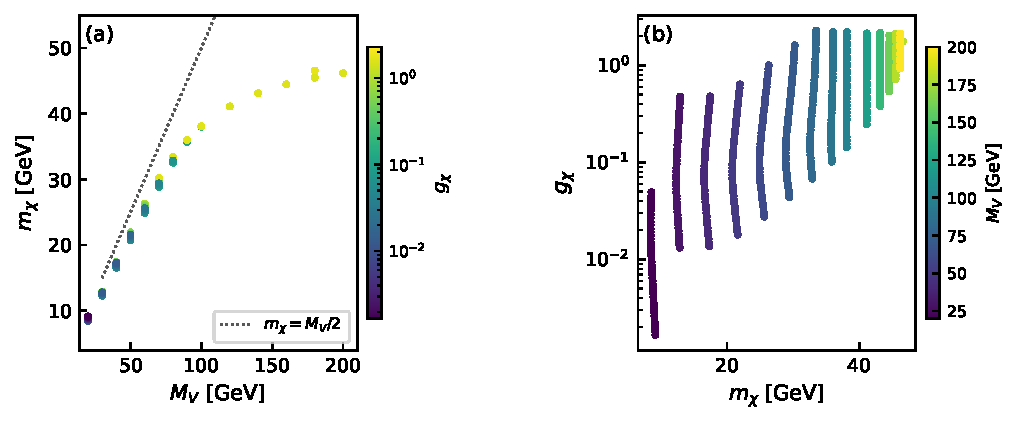
\includegraphics[width=\textwidth]{figs/fig1_v10.pdf}
\caption{The 470 admissible points in two projections. (a) The $(M_V,m_\chi)$ plane, coloured by $g_\chi$, with the kinematic ceiling $m_\chi=M_V/2$. (b) The $(m_\chi,g_\chi)$ plane, coloured by $M_V$. Each vertical strip is one mediator-mass column: $m_\chi$ changes by at most $8\%$ within a column, less than $1\%$ above 90~GeV, while $g_\chi$ spans a factor of 2 to 36.}
\label{fig:constraints}
\end{figure}

\section{The CMS $t\bar t$+MET analysis}\label{sec:cms}

\subsection{Signal generation and event selection}

Signal events are generated at leading order with \textsc{MadGraph5\_aMC@NLO}~\cite{MG5} in the effective model of Eq.~\eqref{eq:lag}, showered with \textsc{Pythia}~8~\cite{PYTHIA} and passed through \textsc{Delphes}~\cite{DELPHES} with a CMS-like detector card. For each point we generate between $8\times10^3$ and $2\times10^4$ events, the larger samples being reserved for points with a sizeable invisible branching ratio, for a total of about $8.3\times10^6$ events. The cross section is computed separately at every point, $0.0022\le\sigma\le10.93$~pb with an integration uncertainty of $0.20$--$0.38\%$; no $g_t^2$ rescaling is used anywhere in the analysis. The cross section already contains the invisible branching ratio of the mediator, so the signal yield is
\begin{equation}
N_{\rm SR}=\mathcal{L}\,\varepsilon_{\rm SR}\,\sigma_{\rm vis},
\qquad
\mathcal{L}=138\ \mathrm{fb}^{-1}=1.38\times10^{5}\ \mathrm{pb}^{-1},
\label{eq:nsr}
\end{equation}
\noindent so that with $\sigma_{\rm vis}$ in pb the yield is $1.38\times10^{5}\,\varepsilon_{\rm SR}\,\sigma_{\rm vis}$. Here $\sigma_{\rm vis}\equiv\sigma_{\rm MG5}$ is the leading-order cross section of the generated process, $pp\to t\bar t\,\chi_1\chi_2\to(bjj)(\bar bjj)\,\chi_1\chi_2$, with both tops decaying hadronically; the width entering the $V$ propagator is the total width, so the factor $\Gamma_{\rm inv}/\Gamma_{\rm tot}$ is already contained in the cross section.
The efficiency $\varepsilon_{\rm SR}$ is that of the seven selection requirements of Table~\ref{tab:sel} (Appendix~\ref{app:sel}). The efficiencies range from $0.66\%$ to $6.59\%$ across the grid. Table~\ref{tab:eff} lists them column by column together with the fraction of events that pass the $p_T^{\rm miss}>250$~GeV requirement, which rises from 1.2\% at 20~GeV to 8.4\% at 200~GeV. The two quantities rise together across the fourteen columns.



The selected events are binned in $p_T^{\rm miss}$ in the fifteen bins of the published post-fit distribution for the all-hadronic $0\ell2b$ signal region: 20~GeV wide from 250 to 530~GeV, with the last bin collecting the overflow above 530~GeV. We adopt those fifteen $p_T^{\rm miss}$ edges unchanged. They are the binning of the published post-fit distribution, not the binning in which CMS performs its fit: CMS extracts the signal with neural-network score bins, and the $p_T^{\rm miss}$ histogram is the projection we use.

\subsection{Signal yields}

The yields span more than two orders of magnitude. At $M_V=50$~GeV and $g_t=0.15$ the efficiency is about $1.8\%$ and the cross section about $0.12$~pb, giving $N_{\rm SR}\approx290$; at $M_V=140$~GeV and $g_t=0.94$ the cross section is $1.30$~pb and the efficiency $4.5\%$, giving $N_{\rm SR}\approx8\times10^3$. The two examples differ in both $M_V$ and $g_t$, so they show the range of yields across the scan rather than the dependence on either variable alone. Column by column, the median efficiency grows with the mediator mass, from $0.87\%$ at 20~GeV to $6.2\%$ at 200~GeV (Table~\ref{tab:eff}), and the cross sections of the heavier columns are larger as well, so both ingredients grow with $M_V$ over this range, and the yields quoted below are the generated ones.

\subsection{Statistical interpretation}

The expected limit is obtained from a binned Poisson likelihood with a single background nuisance parameter that shifts all bins coherently,
\begin{equation}
-2\ln L(\mu,\theta)=\sum_{i=1}^{15}2\left[b_i(1+\theta)+\mu s_i-n_i\ln\!\big(b_i(1+\theta)+\mu s_i\big)\right]+\left(\frac{\theta}{w}\right)^2,
\label{eq:lik}
\end{equation}
where $b_i$ are the CMS post-fit background yields, $s_i$ the signal template of the point under study, $n_i$ the Asimov data $n_i=b_i$, and $w=3.198\%$ the quadrature sum of the background uncertainties divided by the total background. The nuisance parameter is profiled numerically at each $\mu$: a one-dimensional grid in $\theta$ is scanned and the minimum refined by a parabola, and the 95\% CL limit $\mu_{95}$ is then defined by $\mathrm{CL}_s=0.05$ with the asymptotic formulae of Refs.~\cite{CLS,CCGV}. We model the background with a single coherent normalisation nuisance parameter across the fifteen $p_T^{\rm miss}$ bins. A point is called excluded when $\mu_{95}<1$. The grid spans $[-3w,3w]$; an independent minimisation that includes every point with $0.85<\mu_{95}<1.15$ agrees with the tabulated limits to better than $0.2\%$.

The background and data inputs are the published post-fit distributions of the CMS analysis. Fig.~\ref{fig:cmsinput} reproduces them; they are the experimental input to the likelihood. The total background is $9642.0$ events and the observed count is $10224$ in the fifteen bins. We use the observed distribution only to display the input; all limits quoted in this paper are expected limits.

\section{Results: the exclusion region}\label{sec:results}

\subsection{The 470-point physical grid}

Applying the likelihood of Eq.~\eqref{eq:lik} to the 470 points gives an expected limit that ranges from $\mu_{95}=0.00315$ at the heaviest mediator to the numerical cap of the scan, $\mu_{95}=64$, at the weakest coupling of the lightest one, a span of more than four orders of magnitude. The cap is a lower bound imposed by the likelihood scan and not a measured value. \textbf{381 points are excluded at 95\% CL and 89 survive, 43 of them in the $M_V=20$~GeV column.} Every point at or above 100~GeV is excluded. From 30 to 90~GeV the excluded region occupies the coupling range above $g_t\approx0.17$, except for the last few points of the 30 and 40~GeV columns, where the window closes (Table~\ref{tab:columns}). Only at 20~GeV is the column dominated by survivors, and there the single nominally excluded point sits at $g_t=0.249$ and lies within one standard deviation of unity once the Monte Carlo uncertainty of the template is propagated (Section~\ref{sec:sys}); no exclusion is established at 20~GeV.

The classification above is nominal: a point is excluded when $\mu_{95}<1$. Requiring $\mu_{95}+2\sigma_{\rm MC}<1$, with the Monte Carlo uncertainty of each template propagated as in Section~\ref{sec:sys}, turns this into a two-standard-deviation statement. The test was carried out for the 132 points at 20--40~GeV, where the selected yields are smallest; no such test was performed for the remaining 338 points. For those 132 the nominal 1, 34 and 36 exclusions at 20, 30 and 40~GeV become 0, 32 and 32, and the single point at 20~GeV, two at 30~GeV and four at 40~GeV sit within $2\sigma$ of the boundary. Points with $\mu_{95}<0.3$ are unaffected at the quoted precision. We therefore quote the nominal counts in Table~\ref{tab:columns} and give the robust subset separately.

Table~\ref{tab:columns} breaks the result down by mediator mass. The fraction of excluded points is 1/44 at 20~GeV, rises to 34/44 at 30~GeV and 36/44 at 40~GeV, stays at 37--38 of 44 through 50--80~GeV, and reaches unity at 100~GeV and above, while the smallest limit in each column falls from $1.6\times10^{-2}$ at 90~GeV to $3.2\times10^{-3}$ at 200~GeV. The excluded region is therefore not a wedge that closes with mass: it is bounded from below by a nearly horizontal line across the whole mass range, and its upper boundary survives only where the invisible width collapses inside the scanned coupling range.

\begin{table}[t]
\centering
\caption{Expected limits by mediator-mass column. The last two columns give the smallest and largest $\mu_{95}$ within the column; the entry $64$ marks the numerical cap of the likelihood scan and is a lower bound rather than a measured value. The surviving points are those with nominal $\mu_{95}>1$.}
\label{tab:columns}
\begin{tabular}{cccccc}
\toprule
$M_V$ [GeV] & points & excluded & surviving & largest surviving $g_t$ & $\mu_{95}$ range \\
\midrule
 20 & 44 & 1 & 43 & 3.5449 & 0.938--64 \\
 30 & 44 & 34 & 10 & 3.5449 & 0.099--2.93 \\
 40 & 44 & 36 & 8 & 3.5449 & 0.105--3.21 \\
 50 & 44 & 37 & 7 & 0.1645 & 0.085--2.58 \\
 60 & 44 & 38 & 6 & 0.1514 & 0.055--3.11 \\
 70 & 44 & 37 & 7 & 0.1645 & 0.031--2.67 \\
 80 & 43 & 37 & 6 & 0.1650 & 0.023--2.70 \\
 90 & 38 & 36 & 2 & 0.1790 & 0.017--1.05 \\
100 & 34 & 34 & 0 & --- & 0.011--0.61 \\
120 & 27 & 27 & 0 & --- & 0.007--0.20 \\
140 & 22 & 22 & 0 & --- & 0.005--0.10 \\
160 & 17 & 17 & 0 & --- & 0.003--0.04 \\
180 & 14 & 14 & 0 & --- & 0.004--0.03 \\
200 & 11 & 11 & 0 & --- & 0.003--0.02 \\
\bottomrule
\end{tabular}
\end{table}

\subsection{The exclusion boundary}

Figure~\ref{fig:map} is the main result of the paper. Every coloured rectangle is one computed point: the cell spans the logarithmic midpoints between neighbouring $g_t$ values of the same column and the midpoints between neighbouring $M_V$ columns, so no colour is interpolated in either direction and nothing is drawn outside the computed range of a column. The colour encodes $\mu_{95}$ at the central abundance solution and the cells are the points at which the likelihood was evaluated. Of the $14\times44=616$ coordinates in the frame, 470 are computed, 51 have no root of the abundance equation at the fixed mass splitting $\Delta m=1$~MeV used in the recoil normalisation, and 95 have a root but violate $\Gamma_V/M_V<3\%$, where the narrow-width treatment does not apply (58 of these also fail $M_V-2m_\chi\ge5\Gamma_V$). All 146 grey cells lie at $M_V\ge80$~GeV with $g_t\le1.42$; neither kind is an allowed region, and every coordinate inside the frame has been evaluated.

\begin{figure}[t]
\centering
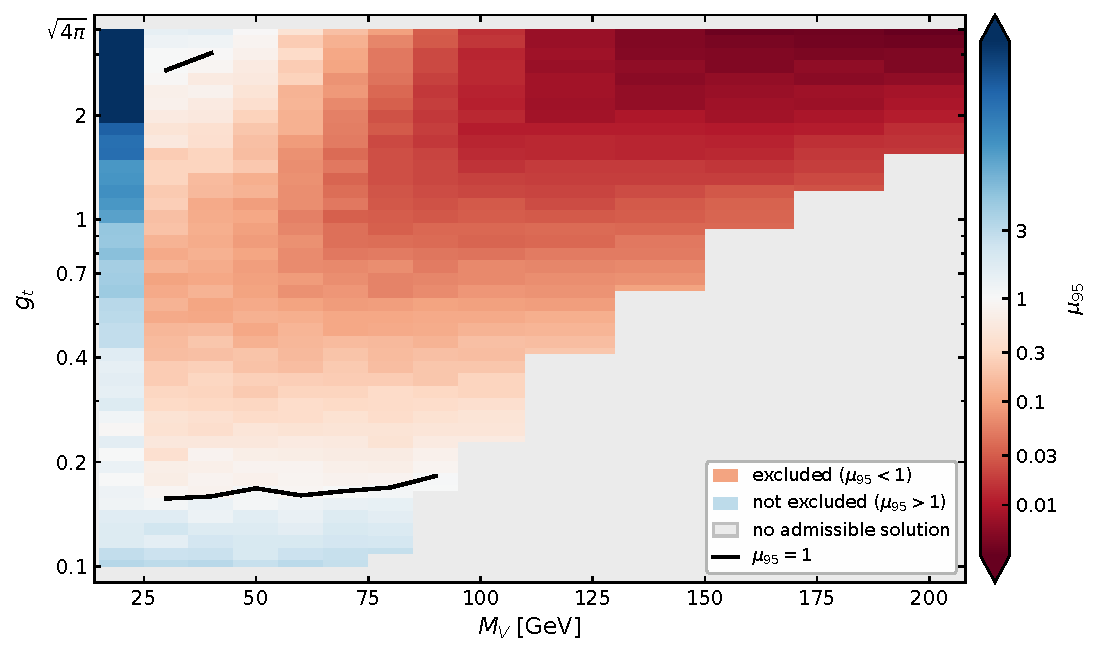
\includegraphics[width=0.88\textwidth]{figs/fig2_v10.pdf}
\caption{Expected CMS $t\bar t$+MET 95\% CL limits on the branch satisfying the recoil-yield, central-abundance and narrow-width conditions, at $\sqrt{s}=13$~TeV with $138\ \mathrm{fb}^{-1}$. Each cell is one computed grid point and no colour is interpolated; red is $\mu_{95}<1$, blue $\mu_{95}>1$, and the neutral tone marks unity. The black line joins the nominal $\mu_{95}=1$ crossings of adjacent columns and is interrupted where the crossing moves by more than a factor 1.5 between them. Grey cells have no admissible solution; circles mark cells at the scan cap, $\mu_{95}=64$.}
\label{fig:map}
\end{figure}

The boundary has two pieces. A lower envelope, nearly flat at $g_t\approx0.15$--$0.19$, runs from 30 to about 90~GeV and separates the production-limited region beneath it; the 20~GeV column has its boundary at $g_t\approx0.24$ with a single point above it; above 100~GeV even the smallest admissible coupling is excluded, so the envelope ends there. An upper edge appears only where the invisible branching ratio falls steeply inside the scanned range: at $g_t\approx2.7$ and $3.0$ for 30 and 40~GeV the window closes and the last computed points return above unity, while from 50 to 90~GeV no such collapse occurs inside $g_t\le\sqrt{4\pi}$ and the excluded region extends to the top of each column. At 20~GeV a single point near $g_t\approx0.25$ is nominally excluded but lies within the Monte Carlo uncertainty of the boundary, so it is not a resolved edge. The closure would move by more than a factor of ten between the 20 and 30~GeV columns with no computed point between them, and no line is drawn across that interval. The points closest to the lower boundary are 1008 ($\mu_{95}=1.000$), 227 ($1.010$) and 2061 ($1.010$), the smallest distance to unity being $0.03\%$, far below the systematic band of Section~\ref{sec:sys}.


\subsection{The two coupling regimes}

Figure~\ref{fig:curves} shows the expected limit as a function of $g_t$ for several mediator masses. Over most of the scanned range the limit falls steeply: the cross section grows roughly as $g_t^2$, so each step in coupling gives a proportionally larger signal. The fall flattens at large $g_t$ and, in the heavier columns, reverses. At $M_V=100$~GeV, the column with the clearest turnover among those shown in Fig.~\ref{fig:curves}, the limit flattens at $\mu_{95}\approx0.013$ between $g_t=2.5$ and $3.3$ and then rises to $0.016$ at $g_t=3.55$, by which point the invisible branching ratio has fallen to $0.14$. The mediator is increasingly decaying into quarks, and the fraction of its decays that produces missing momentum shrinks accordingly.

The same competition is visible more sharply at low mass: at $M_V=30$~GeV the excluded window runs from $g_t\approx0.16$ to $2.7$, with the limit falling from $1.0$ at the lower edge to $0.10$ at its minimum and rising again to $1.45$ at the largest scanned coupling. The turnover is decisive only below 50~GeV: at 30 and 40~GeV it closes the window at $g_t\approx2.7$ and $3.0$. From 50 to 90~GeV the same competition never brings the limit back above unity anywhere inside $g_t\le\sqrt{4\pi}$, so the excluded band continues to the largest admissible coupling, and the top of the coloured region in Fig.~\ref{fig:map} is the upper end of the scanned coupling range, $g_t=\sqrt{4\pi}$, rather than a boundary of the model. The invisibility penalty is visible as a flattening and a partial recovery of the limit; it closes the window only at 30 and 40~GeV, where the recovery reaches unity.

\begin{figure}[htbp]
\centering
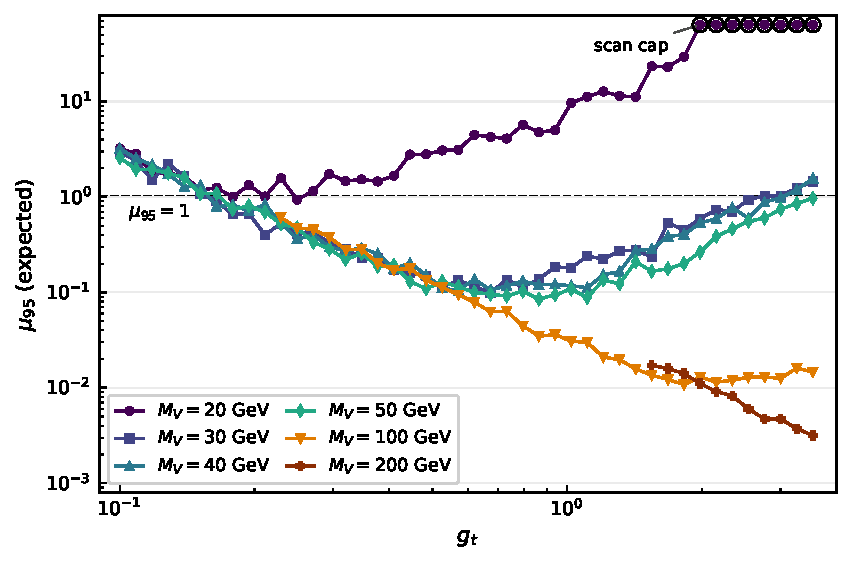
\includegraphics[width=0.84\textwidth]{figs/fig3_v10.pdf}
\caption{Expected limit $\mu_{95}$ as a function of $g_t$ for six mediator masses. The dashed line is $\mu_{95}=1$. The 30 and 40~GeV curves fall below unity, turn over and return above it at $g_t\approx2.7$ and $3.0$, closing the excluded window; from 50~GeV upward the recovery does not reach unity inside $g_t\le\sqrt{4\pi}$; at 20~GeV the limit fluctuates about unity and the exclusion is not resolved. Open circles mark points at the numerical cap, $\mu_{95}=64$.}
\label{fig:curves}
\end{figure}

Whether the turnover actually reopens the window is decided by the absolute level of the signal at the largest coupling, not by the size of the drop. The yield is $N_{\rm SR}=138000\,\varepsilon\,\sigma_{\rm vis}$, and $\varepsilon$ itself grows with $M_V$ (Table~\ref{tab:eff}): the same cross section therefore gives a larger signal in a heavier column. Figure~\ref{fig:vis} shows the two ingredients. At $M_V=20$~GeV the visible cross section falls by a factor 111 between its peak and $g_t=\sqrt{4\pi}$, and the column reopens at $g_t\approx0.25$. At 30 and 40~GeV it falls by a factor of 13 and 15 and the last points land at $\sigma_{\rm vis}\approx0.13$ and $0.10$~pb, where the yield falls below the level the likelihood excludes at 95\% CL and the expected limit returns above unity. At 50~GeV the drop is of the same order, 11, but the efficiency is twice as large as at 30~GeV, so the same cross section produces twice the signal and the column stays excluded all the way to $\sqrt{4\pi}$. The exclusion is set by the signal yield, its fifteen-bin shape and the likelihood, not by the cross section alone; the cross-section level quotes where the turnover lands relative to that combination. The upper boundary is thus a property of $\varepsilon\sigma_{\rm vis}$, not of $\mathrm{BR_{inv}}$ alone.

\begin{figure}[htbp]
\centering
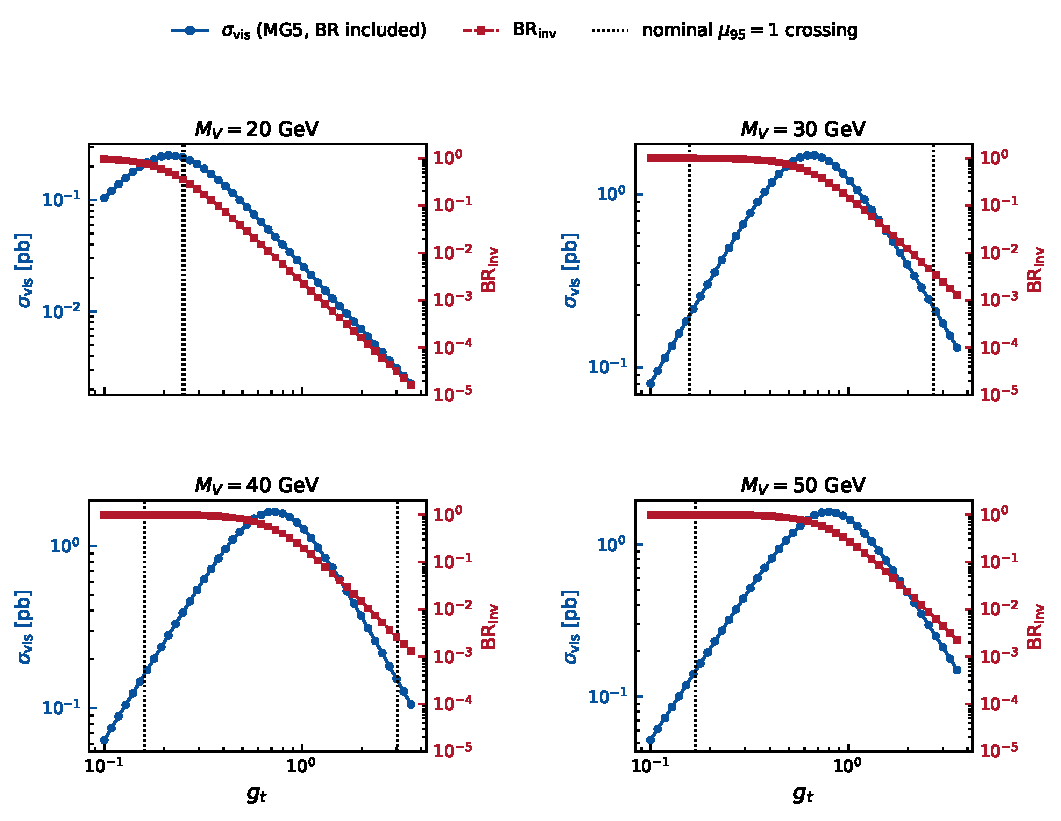
\includegraphics[width=0.97\textwidth]{figs/fig4_v10.pdf}
\caption{Visible cross section $\sigma_{\rm vis}$ (blue, left axis; MadGraph at leading order with the invisible decay of the mediator already included) and invisible branching ratio $\mathrm{BR_{inv}}$ (red, right axis) as a function of $g_t$, for four mediator masses. Dotted vertical lines mark the nominal $\mu_{95}=1$ crossings of each column. The cross section turns over in every column as $\mathrm{BR_{inv}}$ falls; whether the column reopens depends on where the turnover lands relative to the exclusion threshold, that is on $\varepsilon(M_V)\,\sigma_{\rm vis}$, not on the depth of the drop alone.}
\label{fig:vis}
\end{figure}

\FloatBarrier

\section{Stability of the boundary under the Planck window}\label{sec:window}

The exclusion region of Fig.~\ref{fig:map} is computed at the central abundance, $\Omega_\chi h^2=0.1200$. We adopt the abundance window $0.1176\le\Omega_\chi h^2\le0.1224$, a $\pm2\%$ interval around the central value that contains the $\pm1\sigma$ measurement uncertainty, and ask whether motion inside it changes the CMS classification of a node. The relic equation is solved at both edges for every admissible node, and the efficiency is tested with dedicated samples at four of them.

\subsection{The window at every node}

At the two edges the number of nodes passing the validity conditions of Eq.~\eqref{eq:cuts} is $470$ at $0.1176$ and $471$ at $0.1224$, against $470$ at the centre, and the three sets share exactly the central $470$. The single extra record at the high edge sits on the width cut and does not enter the map, which is drawn at the central abundance. The root is refined by bisection until the residual in $\Omega_\chi h^2$ falls below $10^{-5}$, and a node is retained only if $|{\Omega_\chi h^2}/{\rm target}-1|<5\times10^{-3}$, a tolerance carried by the validity flag. The window maps each node into a band of $8$--$223$~MeV in dark mass, with a median of $39$~MeV, always with the higher abundance giving the lighter state; its magnitude is $0.07\%$ of $m_\chi$ at the median and $0.21\%$ at the ninetieth percentile. The coupling moves by $0.14\%$ at the median, $0.55\%$ at the ninetieth percentile and $0.67\%$ at most.

A single branch carries every node. Sampling the relic curve on a $400$-point logarithmic grid at each of the three abundances gives exactly one sign change at every node examined this way, and away from the root the curve never approaches the target more closely than $1.1\%$ of it; within the range we searched, we find no second branch. The yield is $\varepsilon\,\sigma_{\rm vis}$ and, at fixed $g_t$, the cross section tracks the invisible branching ratio, so the window moves the limit by the change in $\mathrm{BR_{inv}}$ plus at most half a per cent from phase space and efficiency — the efficiency term being the one checked at the four nodes of Section~\ref{sec:endpoints}: $0.02\%$ at the median and $0.56\%$ at most across the grid.

Of the three nodes nearest the threshold, 227 has a branching ratio constant to five decimals across the window and does not move, staying at $\mu_{95}=1.0095$; 2061 behaves the same way at $1.0105$; 1008, whose branching ratio changes by $0.05\%$, moves from $1.0003$ to $0.9998$ and $1.0008$ and crosses. That crossing is an order of magnitude below the $2$--$4\%$ Monte Carlo uncertainty of its template, so the classification of 1008 is set by sample size rather than by the window. Every other point lies farther from the boundary than the largest shift its own two edges produce.

\subsection{The four representative nodes}\label{sec:endpoints}

The relic solve fixes the parameters; the efficiency, which is measured from generated events, is tested with dedicated samples at both edges for four nodes: 138 ($M_V=50$~GeV, $g_t=0.1514$), the survivor closest to unity at the time the samples were defined, $\mu_{95}=1.077$; 139 ($M_V=50$~GeV, $g_t=0.1645$), the next, at $1.085$, deliberately adjacent since the two are the only points within $10\%$ of unity in that set; 272 ($M_V=80$~GeV, $g_t=0.1788$), the closest to unity in the $80$--$120$~GeV range, $\mu_{95}=0.800$, where the yield is largest and the mass shift smallest; and 468 ($M_V=140$~GeV, $g_t=0.9397$), a deeply excluded control at $0.0365$. The samples use the same generator chain, the same seven requirements and the same likelihood as the central points; 138 and 139 carry $10^5$ events per edge in two independent halves, 272 and 468 $2\times10^4$. Table~\ref{tab:endpoints} gives the results together with the selection efficiency of each sample, the quantity that limits the comparison.

\subsection{What the endpoint comparison measures}

Three effects separate a centre from an edge. The relic window moves $m_\chi$ by at most $0.23\%$ and the visible cross section by at most $0.5\%$. The finite sample carries a binomial efficiency uncertainty, $\sqrt{(1-\varepsilon)/(N_{\rm gen}\varepsilon)}$, of about $2.4\%$ relative at $10^5$ events and $4.3\%$ at $2\times10^4$, that is $0.04$ and $0.11$ percentage points. The likelihood scales as $\mu_{95}\propto1/N_{\rm SR}$ near the boundary, so a $5\%$ yield difference produces a $5$--$10\%$ change in the limit.

The measured efficiency differences from the centre are $0.98\sigma$ (138, low-$\Omega$), $0.95\sigma$ (138, high-$\Omega$), $0.72\sigma$ (139, low), $1.52\sigma$ (139, high), $2.25\sigma$ (272, low), $0.16\sigma$ (272, high) and $0.24\sigma$/$0.17\sigma$ (468), all consistent with statistics apart from node 272 at the low-abundance edge. That $2.7\sigma$ deficit is already present in the leading MET requirement; the three cards differ only in the random seed, the cross sections agree to $0.3\%$, the central sample reproduces its cutflow on re-analysis, and each sample scatters by $1.5$--$5\%$ when split in half. It is a fluctuation of the event sample, and it is why the comparison resolves shifts of about $10\%$ rather than one per cent.

At these four nodes the window moves the parameters by less than $0.25\%$ in mass and $0.5\%$ in cross section. Node 138 remains on the surviving side: its two edges, $1.231\pm0.060$ and $1.229\pm0.062$, are farther from unity than the centre value $1.077$. Node 139 sits within $1.5\sigma$ of unity at the centre, and its two edges differ from it by less than the sample-to-sample efficiency uncertainty, so its classification is unresolved rather than changed. Node 272 remains excluded: its low-abundance edge, $0.923\pm0.086$, is nominally below unity but only $0.9\sigma$ from it, while its high-abundance edge is $0.863\pm0.080$. Node 468 stays far from the boundary: its limit moves from $0.0365$ at the centre to $0.0380$ and $0.0422$ at the two edges, a $4$--$16\%$ change that leaves all three values deep in the excluded region.

\begin{table}[htbp]
\centering
\caption{Expected limit at the two edges of the Planck window, with the selection efficiency of each sample. Centre values come from the frozen $2\times10^4$-event samples, evaluated with the same likelihood. Edges for 138 and 139 use $10^5$ events in two independent halves; those for 272 and 468 use $2\times10^4$. The errors on $\mu_{95}$ are the RMS of 200 Poisson resamplings of the fifteen bin contents, so they include the fluctuation of the total yield as well as of the shape; the systematic efficiency uncertainty is not included and is quoted separately in the tables.}
\label{tab:endpoints}
\begin{tabular}{lcccccc}
\toprule
& \multicolumn{2}{c}{centre} & \multicolumn{2}{c}{low-$\Omega$ edge} & \multicolumn{2}{c}{high-$\Omega$ edge} \\
\cmidrule(lr){2-3}\cmidrule(lr){4-5}\cmidrule(lr){6-7}
Node & $\varepsilon$ [\%] & $\mu_{95}$ & $\varepsilon$ [\%] & $\mu_{95}$ & $\varepsilon$ [\%] & $\mu_{95}$ \\
\midrule
138 & 1.760 & 1.077 & 1.662 & $1.231\pm0.060$ & 1.665 & $1.229\pm0.062$ \\
139 & 1.575 & 1.085 & 1.646 & $1.012\pm0.049$ & 1.727 & $0.967\pm0.046$ \\
272 & 2.655 & 0.800 & 2.305 & $0.923\pm0.086$ & 2.680 & $0.863\pm0.080$ \\
468 & 4.510 & 0.0365 & 4.560 & $0.0380\pm0.0027$ & 4.545 & $0.0422\pm0.0026$ \\
\bottomrule
\end{tabular}
\end{table}

The relic solve covers all $470$ nodes and the efficiency sample covers four. For the $470$ the window moves one node across the boundary, 1008, by $0.05\%$ and far inside its own statistical uncertainty; that statement rests on the branching-ratio change alone. What the four-node sample adds is narrower: it shows that the efficiency measured at the edges does not differ from the centre beyond its statistical scatter, which is what licenses treating $\varepsilon$ as unchanged in the other columns. It does not verify those columns individually. Reaching a $1\%$ resolution on $\mu_{95}$ at the edges would require of order $4\times10^{2}$ times the events used here at every surviving point.

\section{Systematic uncertainties and limitations}\label{sec:sys}

\subsection{Uncertainties on the expected limit}

Table~\ref{tab:syst} collects the shifts of $\mu_{95}$ obtained by varying one ingredient at a time. The largest effect is the renormalisation and factorisation scale. Nine combinations of $\mu_R$ and $\mu_F$ around the central choice change the cross section by $-21\%$ to $+39\%$, and the limit by $-29\%$ to $+28\%$, which is about one grid step in $g_t$ and moves six points across the boundary in each direction. The scale band is the dominant theory uncertainty and is larger than every other entry in the table.

The remaining entries are an order of magnitude smaller and are collected in Table~\ref{tab:syst}. Of these, the detector efficiency and the xenon normalisation are the only entries that can move a point across the boundary. The efficiency enters the yield linearly, so a $10\%$ variation moves the limit by $9.1\%$. The xenon normalisation enters only through the invisible branching ratio: a $10\%$ change in $\kappa$ changes $g_\chi$ by $10\%$, hence ${\rm BR_{inv}}$ by $0.2\%$ where ${\rm BR_{inv}}\simeq1$ and by up to $21\%$ where ${\rm BR_{inv}}\ll1$. Eleven points lie close enough to the boundary for such a shift to change their classification — three each at 20, 30 and 40~GeV and two at 50~GeV, all with ${\rm BR_{inv}}\le0.68$ — while the points nearest unity outside those columns have ${\rm BR_{inv}}\simeq1$ and move by less than $0.1\%$. The Monte Carlo statistics of the templates and the mediator width contribute at the few-percent level or below for the original grid, where each column carries between $10^2$ and $10^4$ selected events. For the new low-mass columns the selected yields fall to a few hundred events, and the statistical uncertainty of the limit itself becomes the dominant effect near the boundary: resampling the 15-bin template with Poisson fluctuations 150 times and recomputing the limit gives a spread of $0.10$--$0.16$ in $\mu_{95}$ at $M_V=20$~GeV, compared with $0.03$ at $M_V=100$~GeV. At these yields a positive fluctuation of the fitted signal strength inflates $p_b$ in the CLs ratio, which biases the resampled limits low; we do not correct for it and rely on the $2\sigma$ margin instead. We therefore classify a point as excluded only when $\mu_{95}+2\sigma_{\rm MC}<1$: this leaves 32 of 44 points at $M_V=30$~GeV and 32 of 44 at 40~GeV, removes the single nominal exclusion at $20$~GeV, and leaves five to eight points per column straddling the boundary. Two points, 346 and 565, show a run-to-run scatter of $0.87\%$ and $0.76\%$ in three independent integrations, larger than their nominal integration uncertainty; the tabulated values are retained and the effect on the limit is below one percent.

The parton-distribution uncertainty was estimated at three representative points by reweighting to a next-to-leading-order set with 101 members. The central value moves down by $11$--$13\%$ and the replica spread is $9$--$10\%$. The two numbers are different quantities and are not added: the first is a change of central prediction, the second an uncertainty. Neither was propagated point by point across the grid, and the PDF band is therefore quoted as an estimate rather than as a per-point error.

\begin{table}[htbp]
\centering
\caption{Shift of the expected limit when one ingredient is varied. The scale entry is the envelope of nine renormalisation and factorisation scale combinations evaluated at three points and applied to the whole grid; the PDF entries are evaluated at the same three points and not propagated. The $\kappa$ entry is propagated through $g_\chi\to{\rm BR_{inv}}\to$ signal at fixed $m_\chi$, not as a flat rescaling of the signal.}
\label{tab:syst}
\begin{tabular}{lcc}
\toprule
Source & Variation & $\Delta\mu_{95}/\mu_{95}$ \\
\midrule
Monte Carlo statistics & --- & $6.5\%$ \\
Detector efficiency & $\pm10\%$ & $9.1\%$ \\
Xenon normalisation $\kappa$ & $\pm10\%$ & $\le0.2\%$ (${\rm BR_{inv}}\simeq1$) to $21\%$ (${\rm BR_{inv}}\ll1$) \\
Mediator width and $\mathrm{BR}_{\rm inv}$ & $\pm1\%$ & $1.0\%$ \\
Renormalisation and factorisation scale & $+39\%/-21\%$ & $-29\%/+28\%$ \\
Parton distributions (central shift) & $-11$ to $-13\%$ & not propagated \\
Parton distributions (replica spread) & $9$--$10\%$ & not propagated \\
\bottomrule
\end{tabular}
\end{table}

\subsection{Limitations}

The analysis is an approximate, expected-only recast: no observed exclusion map is presented, and every limit quoted here is an expected one. Several of its ingredients differ from the CMS analysis in ways that matter for the interpretation of the boundary.

The selection is applied to a single signal region, the all-hadronic $0\ell2b$ category, while the CMS result combines three lepton categories. The binning is fifteen equal-width bins in $p_T^{\rm miss}$, while CMS extracts the signal with neural-network score bins. The likelihood has one coherent background nuisance and no control region; the CMS model has many parameters constrained by sidebands. These choices make the limit an estimate rather than a reproduction of the published result.

The detector simulation is parameterised. The $b$ tag is a binary Delphes tagging with an efficiency of about $67\%$ at $30$--$100$~GeV, compared with about $75\%$ for the CMS DeepCSV working point, and a light-flavour mistag rate of $1.3\%$ against about $1\%$. The $b$ jet entering the transverse-mass cut is the highest-$p_T$ tagged jet, whereas CMS uses the jet with the largest DeepCSV discriminator; replacing our choice by a truth-flavour priority changes the decision for $215$ of $7727$ events ($2.8\%$) and the selected yield by $151$ of $7453$ ($2.0\%$), an effect smaller than the scale band but not negligible. There is no pileup simulation, the jet radius is $0.5$ rather than $0.4$, and lepton identification and isolation are approximate.

The grid is a candidate set, not an enumeration: it contains the on-shell branch only (Section~\ref{sec:lz}), so off-shell solutions are neither studied nor excluded. The scan covers $M_V=20$--200~GeV. Below 20~GeV the parameter space is not covered by the present scan: the recoil integral is defined down to $m_\chi=8$~GeV, but no grid was generated there, so no statement is made about $M_V<20$~GeV.

Finally, the released package contains the frozen templates, the published post-fit distribution, the likelihood code and the archived generator cards, but not the event samples; it reproduces the limits rather than the generation.

\section{Conclusions}\label{sec:concl}

The exclusion region of Fig.~\ref{fig:map} is the result of this paper. For an exothermic pseudo-Dirac dark sector whose quark couplings follow the quark masses, a fixed xenon recoil yield and the Planck abundance determine the dark mass and coupling at every $(M_V,g_t)$, and the CMS all-hadronic $t\bar t$+MET search then excludes most of the resulting plane. Of the 470 admissible points, 381 are excluded at 95\% CL and 89 survive, 43 of them in the $M_V=20$~GeV column. At and above 100~GeV the entire scan is excluded, with expected limits reaching $\mu_{95}=0.00315$ at 200~GeV. Between 50 and 90~GeV the exclusion covers the whole scanned coupling range above $g_t\approx0.17$ and is bounded from below only; at 30 and 40~GeV a second boundary closes it at $g_t\approx2.7$--$3.0$; at 20~GeV the nominal exclusion is confined to an interval that the present Monte Carlo statistics cannot resolve.

The boundary has a simple physical reading. On the low-coupling side the signal becomes production-limited and the expected limit climbs through unity. On the high-coupling side the mediator decays increasingly into quarks, the invisible branching ratio at the largest scanned coupling falls from $0.89$ at 200~GeV to $2\times10^{-5}$ at 20~GeV, and the expected limit flattens and turns up: at 30 and 40~GeV this closes the window, from 50 to 90~GeV it turns up without reaching unity inside $g_t\le\sqrt{4\pi}$, and at 20~GeV the closure is not resolved. Where no closure occurs the excluded region runs to the largest couplings allowed by the narrow-width condition, and the production threshold alone carves out the surviving wedge at low mediator mass.

Three tests of different depth support this map. The relic equation was solved at both edges of the Planck window for all 470 admissible nodes, which leaves every one of them admissible and moves the dark mass by $0.07\%$ at the median; the only node the window can move across the boundary is one that was already unresolved. For the same nodes the signal was rescaled by the change in the invisible branching ratio, which shifts the limit by $0.02\%$ at the median. Dedicated endpoint samples at four nodes show that the efficiency carries no systematic shift beyond its statistical scatter, and that the boundary cases move by less than that scatter, one of them (139) sitting too close to unity for the present statistics to classify. Three extensions would sharpen the result: a full off-shell treatment extending the grid below $M_V=20$~GeV, a neural-network binning matched to the CMS extraction, and dedicated generation at the window edges for all surviving points, replacing the argument from measured shifts by a per-point verification. The central result stands on the present computation: within the scanned range the plane is excluded at and above 100~GeV, and the surviving wedge is a small and physically identifiable corner of the parameter space.


\appendix
\section{Event selection}\label{app:sel}

The seven requirements of Table~\ref{tab:sel} are applied in the order shown. The last one uses
the highest-$p_T$ $b$-tagged jet; the alternative of ordering the tagged jets by truth flavour is
discussed in Section~\ref{sec:sys}.

\begin{table}[htbp]
\centering
\caption{Selection requirements of the CMS all-hadronic $0\ell2b$ signal region, applied in the order shown. The last requirement defines the $b$ jet used in the transverse-mass cut; the treatment of that choice is discussed in Section~\ref{sec:sys}.}
\label{tab:sel}
\begin{tabular}{ll}
\toprule
Requirement & Value \\
\midrule
Lepton veto & no electron or muon with $p_T>10$~GeV and $|\eta|<2.4$ \\
Jets & at least three with $p_T>30$~GeV, $|\eta|<2.4$ \\
$b$-tagged jets & at least two \\
Missing transverse momentum & $p_T^{\rm miss}>250$~GeV \\
Leading-jet momentum fraction & $p_T(j_1)/H_T<0.5$ \\
Azimuthal separation & $\min\Delta\phi(j_{1,2},p_T^{\rm miss})>0.8$ \\
Transverse mass & $m_T^b>140$~GeV \\
\bottomrule
\end{tabular}
\end{table}

\noindent{\footnotesize Here $H_T$ is the scalar sum of the transverse momenta of the selected jets, and $m_T^b=\sqrt{2\,p_T^{b}p_T^{\rm miss}\left(1-\cos\Delta\phi_{b}\right)}$ with $b$ the highest-$p_T$ $b$-tagged jet among the selected jets, the definition used throughout the analysis.}

\section{Experimental input}\label{app:input}

The expected limits use the published post-fit background and data distributions of the CMS
all-hadronic $0\ell2b$ signal region, reproduced in Fig.~\ref{fig:cmsinput} from
Ref.~\cite{CMS}; the last bin contains the overflow and no aspect of the distributions has been
modified.

\begin{figure}[htbp]
\centering
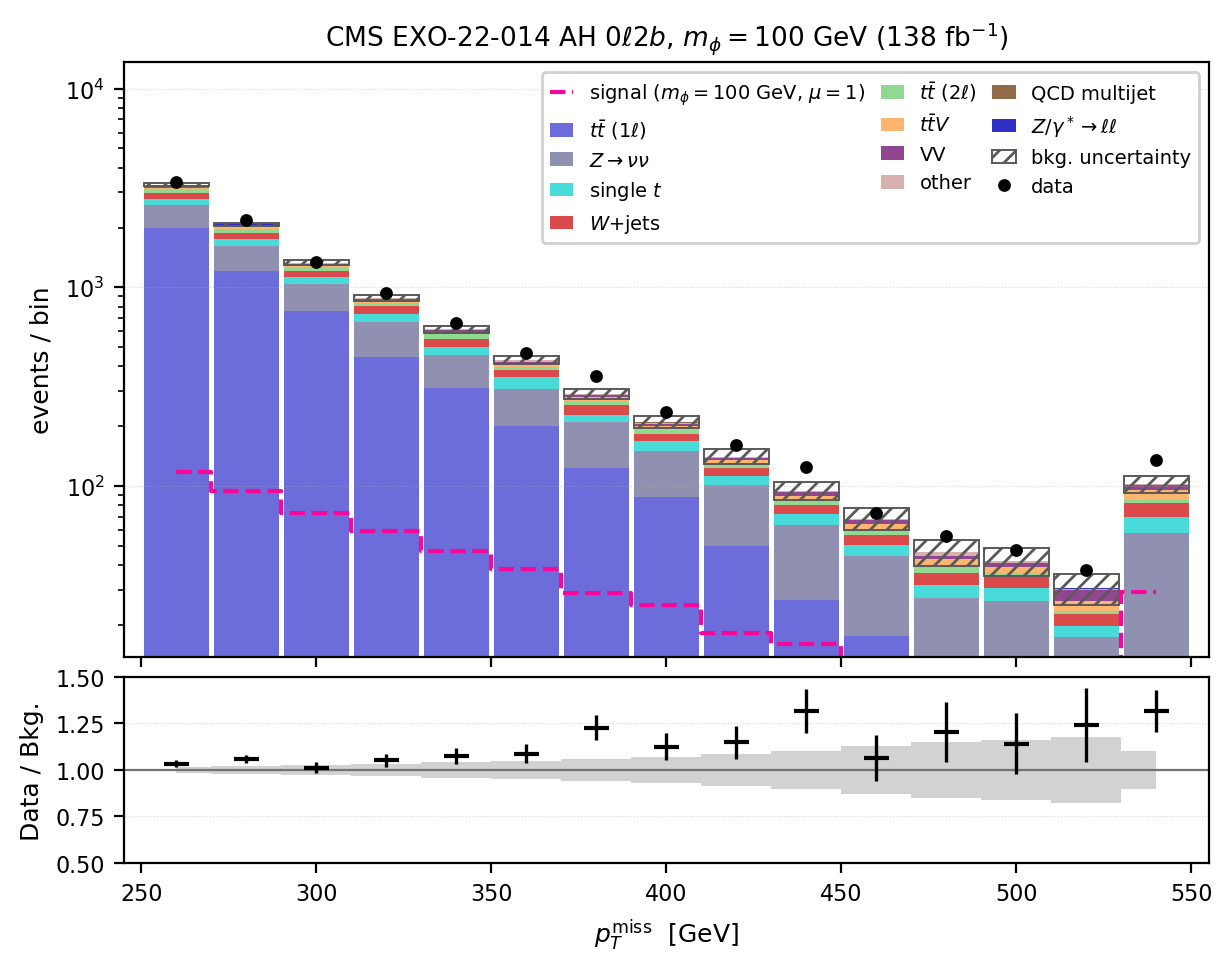
\includegraphics[width=0.64\textwidth]{figs/fig2_cms_inputs.png}
\caption{\textbf{CMS published figure (external input).} Post-fit $p_T^{\rm miss}$
distribution in the CMS all-hadronic $2b$ signal region, reproduced from Ref.~\cite{CMS}.
It is shown to document the background
and data inputs. The last bin contains the overflow events.}
\label{fig:cmsinput}
\end{figure}

\begin{table}[htbp]
\centering
\caption{Selection efficiency by mediator-mass column. The third column gives the minimum, median and maximum efficiency within the column, $\delta\varepsilon$ is the binomial uncertainty at the median point, quoted in percentage points, and the last column is the fraction of generated events that pass the $p_T^{\rm miss}>250$~GeV requirement, applied after the jet, $b$-tag and lepton requirements as listed in Table~\ref{tab:sel}. All 470 points are used.}
\label{tab:eff}
\begin{tabular}{crcccc}
\toprule
$M_V$ [GeV] & points & $\varepsilon$ [\%] (min / median / max) & $\delta\varepsilon$ [percentage points] & $p_T^{\rm miss}>250$ [\%] \\
\midrule
20 & 44 & 0.662 / 0.865 / 1.100 & 0.065 & 1.16 \\
30 & 44 & 0.950 / 1.120 / 1.255 & 0.074 & 1.49 \\
40 & 44 & 1.050 / 1.400 / 1.615 & 0.083 & 1.85 \\
50 & 44 & 1.475 / 1.647 / 1.815 & 0.090 & 2.24 \\
60 & 44 & 1.738 / 1.916 / 2.262 & 0.153 & 2.66 \\
70 & 44 & 2.035 / 2.282 / 2.565 & 0.106 & 3.05 \\
80 & 43 & 2.288 / 2.575 / 2.975 & 0.112 & 3.40 \\
90 & 38 & 2.565 / 2.813 / 3.080 & 0.117 & 3.82 \\
100 & 34 & 2.890 / 3.107 / 3.505 & 0.122 & 4.21 \\
120 & 27 & 3.540 / 3.810 / 4.115 & 0.135 & 5.12 \\
140 & 22 & 4.140 / 4.353 / 4.685 & 0.144 & 5.93 \\
160 & 17 & 4.825 / 5.010 / 5.595 & 0.154 & 6.80 \\
180 & 14 & 5.285 / 5.665 / 6.070 & 0.163 & 7.56 \\
200 & 11 & 5.930 / 6.240 / 6.585 & 0.171 & 8.43 \\
\bottomrule
\end{tabular}
\end{table}


\FloatBarrier
\begin{thebibliography}{99}\small

\bibitem{LZ} LUX-ZEPLIN Collaboration, \emph{Search for dark matter particle interactions in an extended nuclear recoil energy window with the LUX-ZEPLIN (LZ) experiment}, arXiv:2609.02823 [hep-ex].

\bibitem{GHK} C.~Gemmell, D.~Hooper and G.~Krnjaic, \emph{A simple dark matter model to explain the LZ event and Galactic Center excess}, arXiv:2609.26570 [hep-ph].

\bibitem{DHX} X.-Y. Du, W.~Huang and K.~Xie, \emph{Pseudo-Dirac inelastic dark matter in the leptophobic $U(1)_B$ model: confronting the LUX-ZEPLIN high-recoil event with collider searches}, arXiv:2609.07225 [hep-ph].

\bibitem{CMS} CMS Collaboration, \emph{Search for dark matter produced in association with one or two top quarks in proton-proton collisions at $\sqrt{s}=13$~TeV}, JHEP \textbf{08} (2025) 085, doi:10.1007/JHEP08(2025)085 [arXiv:2505.05300 [hep-ex]].

\bibitem{PLANCK} Planck Collaboration, \emph{Planck 2018 results. VI. Cosmological parameters}, Astron.\ Astrophys.\ \textbf{641} (2020) A6, doi:10.1051/0004-6361/201833910 [arXiv:1807.06209 [astro-ph.CO]].

\bibitem{CLS} A.~L.~Read, \emph{Presentation of search results: the $CL_s$ technique}, J.\ Phys.\ G \textbf{28} (2002) 2693, doi:10.1088/0954-3899/28/10/313.

\bibitem{CCGV} G.~Cowan, K.~Cranmer, E.~Gross and O.~Vitells, \emph{Asymptotic formulae for likelihood-based tests of new physics}, Eur.\ Phys.\ J.\ C \textbf{71} (2011) 1554, doi:10.1140/epjc/s10052-011-1554-0 [arXiv:1007.1727 [physics.data-an]].

\bibitem{SHM} M.~C.~Smith \emph{et al.}, \emph{The RAVE survey: constraining the local Galactic escape speed}, Mon.\ Not.\ R.\ Astron.\ Soc.\ \textbf{379} (2007) 755, doi:10.1111/j.1365-2966.2007.11964.x [arXiv:astro-ph/0611671].

\bibitem{HELM} J.~Engel, \emph{Nuclear form factors and WIMP-nucleus elastic scattering}, Phys.\ Lett.\ B \textbf{264} (1991) 114, doi:10.1016/0370-2693(91)90712-Y.

\bibitem{PDG} R.~L.~Workman \emph{et al.} [Particle Data Group], \emph{Review of particle physics}, Prog.\ Theor.\ Exp.\ Phys.\ \textbf{2022} (2022) 083C01, doi:10.1093/ptep/ptac097.

\bibitem{MG5} J.~Alwall \emph{et al.}, \emph{The automated computation of tree-level and next-to-leading order differential cross sections, and their matching to parton shower simulations}, JHEP \textbf{07} (2014) 079, doi:10.1007/JHEP07(2014)079 [arXiv:1405.0301 [hep-ph]].

\bibitem{PYTHIA} T.~Sj\"ostrand \emph{et al.}, \emph{An introduction to PYTHIA 8.2}, Comput.\ Phys.\ Commun.\ \textbf{191} (2015) 159, doi:10.1016/j.cpc.2015.01.024 [arXiv:1410.3012 [hep-ph]].

\bibitem{DELPHES} J.~de~Favereau \emph{et al.}, \emph{DELPHES 3: a modular framework for fast simulation of a generic collider experiment}, JHEP \textbf{02} (2014) 057, doi:10.1007/JHEP02(2014)057 [arXiv:1307.6346 [hep-ex]].

\bibitem{MICROMEGAS} G.~B\'elanger, F.~Boudjema, A.~Pukhov and A.~Semenov, \emph{Dark matter direct detection rate in a generic model with micrOMEGAs 2.2}, Comput.\ Phys.\ Commun.\ \textbf{180} (2009) 747, doi:10.1016/j.cpc.2008.11.019 [arXiv:0803.2360 [hep-ph]].

\end{thebibliography}


\end{document}
